% Provenance (never printed): see sources/outline_sources.md (Year 1: litho-, bio- and
% chronostratigraphy; boundary stratotypes; mass extinctions as global markers; the
% international chart). Exercise and problem values in the Book 3 scratch calculator
% calc/ch24.py; the chart from figdata/bachelor-1/ics_chart.py (shared ics rows).
% The principles of relative dating, eras and periods are Book 1's (g7 geological-time) and
% are re-founded here. Mass extinctions belong to the biology series (recalled in prose);
% their Earth causes are the Year 2 volume's (phanerozoic-earth). Correlation of logs and
% unconformities are ch. 5's; facies ch. 21's; compaction ch. 23's. Radiometric dating is
% ch. 25's. Sequence stratigraphy, facies models and Walther's law are the Year 3 volume's;
% magnetostratigraphy too: prose pointers only. "Transgression" is explained in prose.
\chapter{السلّم الطبقي}\label{ch:b1:stratigraphic-scale}

على شاطئ إتزورون في زوماييا على الساحل الباسكي، تتكوّن الجروف من طبقات رقيقة من الحجر الكلسي والمارل، مائلة ومكرّرة على مئات الأمتار. وعند \omterm{def:b1:geological-maps:geological-map}{تماس} واحد، حيث ينتهي طبقة كلسية شاحبة وتبدأ المارلات الحمراء، يُثبَّت في الصخر قرص برونزي منقوش عليه أربعة أحرف (الشكل أدناه). إنه مسمار ذهبي. فهو يحدّد، لكوكب الأرض كله، اللحظة التي يبدأ عندها أحد أقسام الزمن الجيولوجي، أي \omterm{def:b1:stratigraphic-scale:chronostratigraphy}{الطابق} السيلاندي. والصخر في باتاغونيا أو في سيبيريا يكون سيلانديًّا إن ترسّب بعد اللحظة المسجّلة عند هذا \omterm{def:b1:geological-maps:geological-map}{التماس}، وقبل اللحظة المسجّلة عند المسمار التالي أعلى السلّم. يشرح هذا الفصل كيف احتاج الجيولوجيون إلى مثل هذه العلامة: ثلاث طرق مختلفة لتقسيم كومة من الصخور، والمبادئ التي ترتّبها، والخطوط التي تربط مقاطع متباعدة، والسلّم الدولي الذي يجمع النتيجة.

\begin{omfigure}
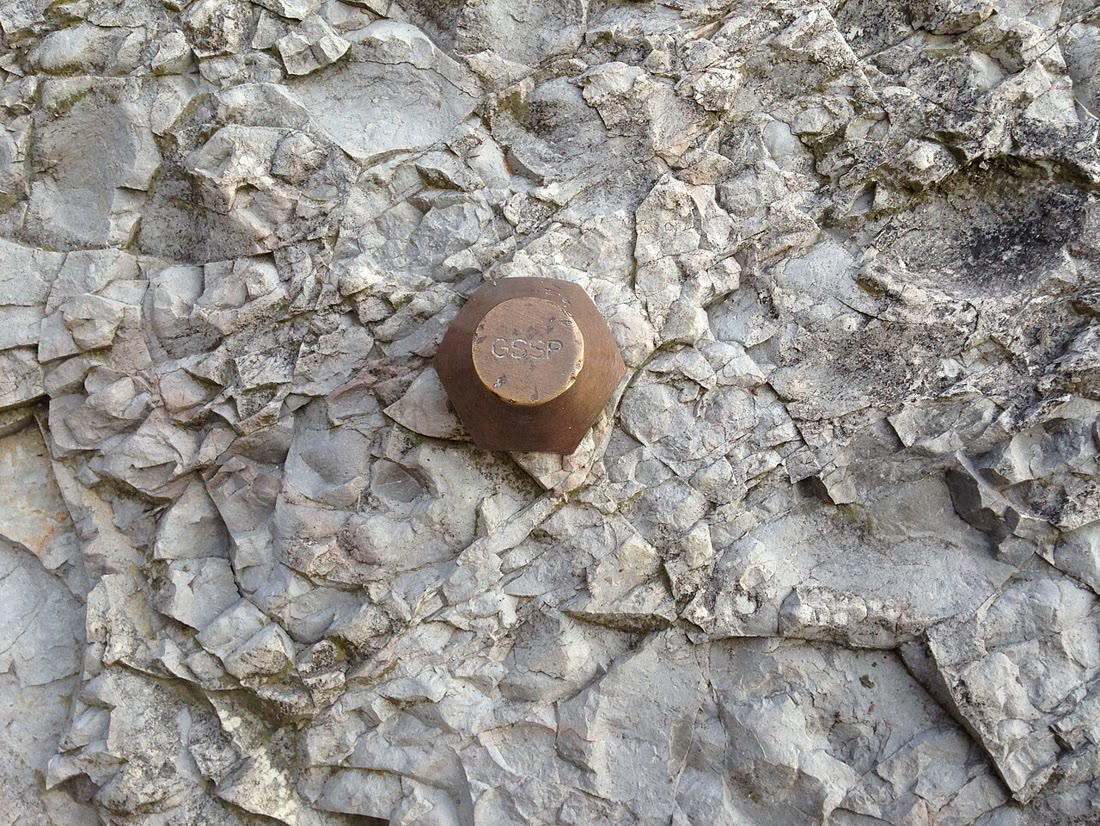
\includegraphics[width=0.62\linewidth]{images/book3/b1-golden-spike-zumaia.jpg}

{\small المسمار الذهبي للطابق السيلاندي في مقطع زوماييا: علامة برونزية منقوش عليها GSSP، عند قمّة أعلى طبقة كلسية من تكوين واحد، عند قاعدة المارل الأحمر للتكوين الذي يليه. (Josugoni, CC BY-SA 4.0, عبر Wikimedia Commons.)}
\label{fig:b1:stratigraphic-scale:zumaia}
\end{omfigure}
% ledger: commons:zumaia-gssp, gssp:selandian

\begin{recall}
في كومة من الطبقات لم تُقلب، كل طبقة أحدث من التي تحتها؛ والبنية التي تقطع الصخور أحدث منها؛ والحفريات تتغيّر من الطبقات الأقدم إلى الأحدث بالترتيب نفسه في كل مكان؛ وتاريخ الأرض مقسّم إلى حقب وعصور جيولوجية، لكل منها عمر بالسنين لبدايتها، تجمعها سلّم دولي (الكتاب الأول، الصف السابع). وسجلّ الحفر يسجّل الوحدات التي ظهرت على عمق معيّن، والترابط يطابق الوحدات نفسها من سجلّ إلى آخر (\cref{def:b1:cross-sections:log})؛ \omterm{def:b1:cross-sections:unconformity}{وعدم التوافق} سطح تآكل أو لا ترسيب (\cref{def:b1:cross-sections:unconformity}). \omterm{def:b1:clastic-sediments:facies}{والسحنة الرسوبية} جسم من صخر تسجّل صفاته بيئته الترسيبية (\cref{def:b1:clastic-sediments:facies}). وتصف كتب الأحياء كيف تظهر الأنواع وتنقرض، والانقراضات الجماعية القليلة التي اختفى فيها جزء كبير من كل الأنواع في زمن قصير.
\end{recall}

\section{ثلاث طرق لتقسيم الصخور}\label{sec:b1:stratigraphic-scale:three}

يستطيع الجيولوجي الذي يُسجّل جرفًا أن يقسّم الكومة نفسها من الطبقات بثلاث طرق: بما تتكوّن منه الصخور، وبالحفريات التي تحويها، وبالزمن الذي رُسّبت خلاله. والتقسيمات الثلاثة تجيب عن أسئلة مختلفة، وحدودها لا تتطابق بالضرورة. وقواعد تسمية كل نوع من الوحدات وتعريفه تضعها اتفاقية دولية.
% ledger: isg:lithostratigraphy

\begin{definition}[التكوين، والعضو، والمجموعة]\label{def:b1:stratigraphic-scale:lithostratigraphy}
\emph{الوحدة الصخرية}\index{الوحدة الصخرية} جسم من صخر يُعرَّف ويُعرف بصخريّته وبموضعه بين أجسام أخرى، مهما كان عمره. والوحدة الأساسية هي \emph{التكوين}\index{التكوين (التصنيف الصخري)}: جسم من الصخر يتميّز بما يكفي عن جيرانه ليُرسم على خريطة بمقياس الإقليم، وتُقسَّم إليه العمودية كلّها. و\emph{العضو}\index{العضو (التصنيف الصخري)} تقسيم مسمّى داخل التكوين، يُميَّز بصخريّته؛ و\emph{المجموعة}\index{المجموعة (التصنيف الصخري)} تتابع من تكوينين أو أكثر لها صفات صخرية مشتركة مهمّة. ويصل الاسم الرسمي اسمًا جغرافيًّا محليًّا بالرتبة أو بالصخر السائد: حجر كِل الرملي، وتكوين مردون الصخري.
\end{definition}
% ledger: isg:lithostratigraphy

قد يكون \omterm{def:b1:stratigraphic-scale:lithostratigraphy}{التكوين} أقلّ من متر في السماكة، أو عدّة آلاف من الأمتار. ويُمدّ بعيدًا عن قطاعه النموذجي بقدر ما تُعرف صخريّته، فتتبع حدوده الصخر، لا الزمن.
% ledger: isg:lithostratigraphy

\begin{definition}[الحيّز الأحيائي، والحفرية الدليلية، ومعطى الظهور الأول]\label{def:b1:stratigraphic-scale:biozone}
\emph{الحيّز الأحيائي}\index{الحيّز الأحيائي} جسم من الطبقات يُعرَّف أو يُوصف بالحفريات التي يحويها. و\emph{حيّز المدى}\index{حيّز المدى} يضمّ الوجودات المعروفة لتصنيف واحد؛ و\emph{حيّز الفاصل}\index{حيّز الفاصل} جسم الطبقات الواقع بين أفقين حفريّين محدّدين، كأدنى الوجودات لتصنيفين. و\emph{معطى الظهور الأول}\index{معطى الظهور الأول} (FAD) لتصنيف هو أفق أدنى وجوداته، و\emph{معطى الظهور الأخير}\index{معطى الظهور الأخير} أفق أعلاها. و\emph{الحفرية الدليلية}\index{الحفرية الدليلية} تصنيف يُستعمل لتمييز حيّز أحيائي: وأفضلها واسعة الانتشار، وفيرة، سهلة التعرّف، وقصيرة العمر.
\end{definition}
% ledger: isg:biostratigraphy, og:stratigraphy-principles

الأفق الحفري لا سماكة له؛ أما \omterm{def:b1:stratigraphic-scale:biozone}{الحيّز الأحيائي} فقد يكون بضعة أمتار أو بضع مئات منها، بحسب سرعة تراكم الرسوب أثناء عيش التصنيفات. ولأن الأنواع تتطوّر ولا تعود بعد انقراضها، فإن تجمّع الحفريات في أيّ عمر فريد. وبعض أفضل الحفريات الدليلية أحافير دقيقة، كالفورامينيفيرا والكونودونتات: واسعة الانتشار، وفيرة، وصغيرة بما يكفي لاستخلاصها من قصاصات بئر.
% ledger: isg:biostratigraphy, og:stratigraphy-principles

\begin{definition}[الوحدات الكرونوستراتغرافية والجيوكرونولوجية]\label{def:b1:stratigraphic-scale:chronostratigraphy}
\emph{الوحدة الكرونوستراتغرافية}\index{الوحدة الكرونوستراتغرافية} هي جسم كل الصخور التي تكوّنت خلال فترة زمنية جيولوجية معيّنة، وخلالها وحدها؛ وحدودها أسطح متساوية العمر. والفترة الزمنية نفسها \emph{وحدة جيوكرونولوجية}\index{الوحدة الجيوكرونولوجية}. والرتب، من الأصغر، هي \emph{الطابق}\index{الطابق (الكرونوستراتغرافي)} (زمنه: عمر)، و\emph{السلسلة}\index{السلسلة (الكرونوستراتغرافي)} (حقبة)، و\emph{النظام}\index{النظام (الكرونوستراتغرافي)} (دورة)، والإراثيم (عصر) والإيونوثيم (إيون)؛ وكل وحدة تتكوّن من عدّة وحدات متتالية من الرتبة التي دونها.
\end{definition}
% ledger: isg:chronostratigraphy

الكلمتان تصفان التقسيم نفسه مرئيًّا كصخر أو كزمن (\cref{tab:b1:stratigraphic-scale:ranks}): فصخور الجوراسي تكوّنت خلال دورة الجوراسي، \omterm{def:b1:stratigraphic-scale:chronostratigraphy}{والسلسلة} الجوراسية السفلى خلال حقبة الجوراسي المبكّرة. \omterm{def:b1:stratigraphic-scale:chronostratigraphy}{والطابق} أصغر وحدة معروفة في كل أنحاء العالم.
% ledger: isg:chronostratigraphy, chart:danian

\begin{table}[htbp]
\centering
\begin{tabular}{lll}
\hline
\omterm{def:b1:stratigraphic-scale:chronostratigraphy}{الوحدة الكرونوستراتغرافية} (الصخر) & \omterm{def:b1:stratigraphic-scale:chronostratigraphy}{الوحدة الجيوكرونولوجية} (الزمن) & المثال \\
\hline
إيونوثيم & إيون & الفانيروزويّ \\
إراثيم & عصر & السينوزويّ \\
نظام & دورة & الباليوجين \\
سلسلة & حقبة & الباليوسين \\
طابق & عمر & الدانيّ (\qtyrange{66.00}{61.66}{\Ma}) \\
\hline
\end{tabular}
\caption{رتب الوحدات الكرونوستراتغرافية والجيوكرونولوجية، مع الوحدات التي تحوي الدانيّ، أول طابق من السينوزويّ.}
\label{tab:b1:stratigraphic-scale:ranks}
\end{table}
% ledger: isg:chronostratigraphy, chart:danian

\section{المبادئ والترابط}\label{sec:b1:stratigraphic-scale:principles}

قبل أن يُؤرَّخ أيّ صخر بالسنين، قُرئ ترتيب الأحداث من الصخور نفسها. وقد وضع نيكولاس ستينو مبادئ علم الطبقات الأساسية عام 1669؛ وبين 1785 و\num{1800} أضاف هاتون وويليام سميث استعمال الطبقات كفترات زمنية، واستعمال حفرياتها للتعرّف عليها.
% ledger: og:stratigraphy-principles, usgs:hutton-smith

\begin{definition}[مبادئ علم الطبقات]\label{def:b1:stratigraphic-scale:principles}
\begin{enumerate}
  \item \emph{مبدأ التراكب}\index{مبدأ التراكب}: في تتابع من الطبقات الرسوبية لم يُقلب، كل طبقة أحدث من التي تستقرّ عليها.
  \item \emph{مبدأ الأفقية الأصلية}\index{مبدأ الأفقية الأصلية}: تُرسَّب الرسوبات وتدفّقات الحمم أفقيًّا، أو قريبًا من ذلك، وتميل قليلًا عند حواف الحوض.
  \item \emph{مبدأ الاستمرار الجانبي}\index{مبدأ الاستمرار الجانبي}: داخل الحوض، تمتدّ الطبقة باستمرار في كل اتجاه حتى تنحسر عند حافة الحوض أو عند عائق؛ والطبقة التي يقطعها واد تستمرّ على الجانب الآخر.
  \item \emph{مبدأ علاقات القطع}\index{مبدأ علاقات القطع}: الجسم أو البنية التي تقطع الصخور، كجدار دايك أو صدع أو سطح تآكل، أحدث من الصخور التي تقطعها.
  \item \emph{مبدأ التعاقب الحيواني}\index{مبدأ التعاقب الحيواني}: تتعاقب التصنيفات الحفرية بالترتيب نفسه في كل إقليم، فالصخور التي تحوي التجمّع نفسه من نفس العمر.
\end{enumerate}
\end{definition}
% ledger: og:stratigraphy-principles, eli:relative-dating, usgs:fossil-succession, isg:chronostratigraphy

ليست المبادئ متساوية القوّة. فالتراكب يعطي ترتيبًا يجب على كل طريقة أخرى أن تحترمه. والأفقية الأصلية هي ما يجعل الطبقة المائلة سجلًّا لتشوّه لاحق. والاستمرار الجانبي هو ما يسمح للجيولوجي برسم الطبقة نفسها على جانبي واد، وفي مسافة محدودة، فإن مستوى الطبقة المتتبّع على الأرض هو أفضل خطّ للعمر نفسه. والتعاقب الحيواني هو المبدأ الذي يعبر المحيطات؛ وهو موضوع الفقرات التالية.
% ledger: isg:chronostratigraphy, og:stratigraphy-principles

\subsection*{الترابط بالحيّزات الأحيائية}

الترابط بالحفريات يقارن ترتيب الظهور الأول والأخير في قطاعين (الشكل أدناه). والاثنان ليسا موثوقين بالمقدار نفسه. فأعلى حفرية لتصنيف وُجدت في قطاع تتوقّف على عدد ما حُفظ منها: فحيث تكون نادرة، قد تقع آخر حفرية وُجدت أسفل المستوى الذي انقرض عنده التصنيف فعلًا، ويمكن أن تظهر حفرية تآكلت وأعيد ترسيبها فوقه. ويمكن أن يُزاح الظهور الأول أيضًا، لكن التصنيف الواسع الانتشار الذي انتشر بسرعة يُصادَف عند المستوى نفسه تقريبًا عبر حوض كامل.
% ledger: isg:biostratigraphy

\begin{omfigure}
\begin{tikzpicture}[font=\footnotesize, y=0.13cm]
  % section 1: 40 m, sandstone 0-14, shale 14-40
  \fill[lith sandstone] (0,0) rectangle (0.8,14);
  \fill[lith shale] (0,14) rectangle (0.8,40);
  \draw[black!70] (0,0) rectangle (0.8,40);
  \node[anchor=south, font=\small] at (1.4,41.5) {القطاع 1};
  \foreach \x/\a/\b/\t in {1.1/0/27/a, 1.4/10/34/b, 1.7/20/40/c, 2.0/30/40/d} {
    \draw[line width=2.2pt, omThm] (\x,\a) -- (\x,\b);
    \node[anchor=base, font=\scriptsize] at (\x,-4.5) {\t};
  }
  \foreach \y/\z in {5/a, 15/b, 25/c, 35/d}
    \node[anchor=east, font=\scriptsize] at (-0.1,\y) {الحيّز \z};
  \foreach \y in {10,20,30} \draw[black!50] (-1.3,\y) -- (0,\y);
  % scale bar
  \draw[thick] (-1.5,0) -- (-1.5,10) node[midway, anchor=east, font=\scriptsize] {\qty{10}{m}};
  % section 2: 24 m, sandstone 0-3, shale 3-24
  \begin{scope}[xshift=7cm]
    \fill[lith sandstone] (0,0) rectangle (0.8,3);
    \fill[lith shale] (0,3) rectangle (0.8,24);
    \draw[black!70] (0,0) rectangle (0.8,24);
    \node[anchor=south, font=\small] at (1.4,25.5) {القطاع 2};
    \foreach \x/\a/\b/\t in {1.1/0/13/a, 1.4/6/20/b, 1.7/12/24/c, 2.0/18/24/d} {
      \draw[line width=2.2pt, omThm] (\x,\a) -- (\x,\b);
      \node[anchor=base, font=\scriptsize] at (\x,-4.5) {\t};
    }
    \foreach \y/\z in {3/a, 9/b, 15/c, 21/d}
      \node[anchor=west, font=\scriptsize] at (2.3,\y) {الحيّز \z};
    \foreach \y in {6,12,18} \draw[black!50] (0.8,\y) -- (2.3,\y);
  \end{scope}
  % correlation of the first appearances
  \foreach \u/\v/\t in {10/6/b, 20/12/c, 30/18/d}
    \draw[densely dashed, omThm!70!black] (2.15,\u) -- (6.85,\v)
      node[pos=0.5, fill=white, inner sep=1pt, font=\scriptsize] {FAD \t};
\end{tikzpicture}

{\small مخطّط المدى والترابط بالحيّزات الأحيائية (تصنيفات خيالية من \emph{a} إلى \emph{d}). الأشرطة السميكة هي مدى التصنيفات في كل قطاع. وتُحدّ ثلاثة حيّزات فاصلة بالظهور الأول ل\emph{b} و\emph{c} و\emph{d}، وهي موصولة من قطاع إلى آخر (متقطّعة). والظهور الأخير ل\emph{a} يقع في الجزء الأعلى من الحيّز~\emph{c} في القطاع~1، وقرب قاعدته في القطاع~2: فهو دليل أضعف. والحيّزات أرقّ في القطاع~2، حيث تراكم الرسوب ببطء أكبر.}
\label{fig:b1:stratigraphic-scale:range-chart}
\end{omfigure}

\begin{method}[ترابط القطاعات بالحيّزات الأحيائية]\label{met:b1:stratigraphic-scale:biozones}
\begin{enumerate}
  \item ارسم لكل قطاع مدى كل تصنيف بدلالة الارتفاع: من أدنى وجوده إلى أعلاه.
  \item اختر الآفاق الحفرية التي تحدّد الحيّزات، ويُفضَّل الظهور الأول لتصنيفات واسعة الانتشار مستقلّة عن السحنة.
  \item ارسم حدود الحيّزات في كل قطاع عند هذه الآفاق.
  \item صِل الآفاق نفسها من قطاع إلى آخر؛ وتحقّق من أن الخطوط لا تتقاطع، كما يقتضي التراكب.
  \item اقرأ، بين خطّين، سماكة كل حيّز في كل قطاع؛ وحيث يغيب حيّز، ابحث عن عدم توافق أو تغيّر في السحنة قبل أن تستنتج غياب التصنيف.
\end{enumerate}
\end{method}

\omterm{def:b1:stratigraphic-scale:biozone}{الحيّز الأحيائي} لا يكون أفضل من استقلال حفرياته عن البيئة. فالمحارة التي عاشت على شواطئ رملية فقط لا تُوجد إلا في الحجر الرملي؛ وتتبّعها من قطاع إلى آخر يتبع الحجر الرملي، لا الزمن. والترابط الأحيائي ليس بالضرورة ترابطًا زمنيًّا: فقد يتبع سحنة يتغيّر عمرها من مكان إلى آخر.
% ledger: isg:biostratigraphy

\subsection*{حدود تعبر الزمن}

ترسَّب رسوبات مختلفة في الزمن نفسه في أماكن مختلفة: الرمل على الشاطئ، والطين في البحر المفتوح، والكلس أبعد على رفّ يفتقر إلى الرمل. ولذلك يعبر خطّ العمر نفسه من صخريّة إلى أخرى. وعلى العكس، فإن حدًّا صخريًّا يُتتبّع عبر حوض لا يلزم أن يكون خطّ عمر متساوٍ البتّة.
% ledger: og:stratigraphy-principles, isg:chronostratigraphy

\begin{definition}[الحدّ المتباين الزمن]\label{def:b1:stratigraphic-scale:diachronous}
يكون الحدّ \emph{متباين الزمن}\index{الحدّ المتباين الزمن} حين يتغيّر عمره من مكان إلى آخر على امتداده. وحدود التكوينات والسحنات متباينة الزمن عادةً؛ أما حدود الوحدات الكرونوستراتغرافية فهي، بالتعريف، ليست كذلك.
\end{definition}
% ledger: isg:lithostratigraphy, isg:chronostratigraphy, isg:biostratigraphy

الحالة الكلاسيكية هي التجاوز البحري: يرتفع \omterm{def:b1:diagenesis-basins:eustasy}{مستوى البحر النسبي} أسرع مما يملأ الرسوب المكان المصنوع، فينتقل الشاطئ نحو اليابسة. ويُرسَّب رمل الشاطئ عند خطّ الشاطئ في كل لحظة، فتنتشر طبقة من الحجر الرملي نحو اليابسة معه؛ وتعلوها طين أعماق البحر. فقمّة الحجر الرملي هي إذن أثر الشاطئ المتحرّك: أحدث نحو اليابسة، وأقدم نحو البحر (الشكل أدناه). وترتيب السحنات في قطاع رأسي واحد، أي حجر رملي تحته صخر طيني تحته حجر كلسي، يكرّر ترتيبها عبر الرفّ في لحظة واحدة؛ والمجلد الثالث يجعل ذلك أساس نماذج سحناته.
% ledger: og:stratigraphy-principles, isg:lithostratigraphy

\begin{omfigure}
\begin{tikzpicture}[font=\footnotesize, x=1cm, y=1cm]
  % basement surface B(x) = 1.6 (1 - x/14), rising towards the land on the left
  \fill[lith granite] (0,-0.5) -- (0,1.6) -- (14,0) -- (14,-0.5) -- cycle;
  \fill[lith sandstone] (0,1.6) -- (14,0) -- (14,0.5) -- (0,2.1) -- cycle;
  \fill[lith shale] (0,2.1) -- (14,0.5) -- (14,1.5) -- (0,3.1) -- cycle;
  \fill[lith limestone] (0,3.1) -- (14,1.5) -- (14,3.6) -- (0,3.6) -- cycle;
  \draw[unconformity] (0,1.6) -- (14,0);
  \draw[black!70] (0,2.1) -- (14,0.5) (0,3.1) -- (14,1.5);
  \draw[black!70] (0,-0.5) rectangle (14,3.6);
  % time lines: horizontal, from the basement (or the left edge) to the right edge
  \foreach \y/\t in {0.6/1, 1.1/2, 1.6/3, 2.1/4, 2.6/5, 3.1/6} {
    \pgfmathsetmacro{\xs}{max(0, 14*(1-\y/1.6))}
    \draw[omThm, thick, densely dashed] (\xs,\y) -- (14,\y) node[anchor=west, text=black] {$t_\t$};
  }
  % two sections
  \foreach \x/\n in {3/1, 11/2} {
    \draw[very thick, black] (\x,-0.5) -- (\x,3.6);
    \node[anchor=south, font=\small] at (\x,3.65) {القطاع \n};
  }
  \node[fill=white, inner sep=1pt, font=\scriptsize] at (5.6,1.21) {حجر رملي};
  \node[fill=white, inner sep=1pt] at (12.6,1.2) {صخر طيني};
  \node[fill=white, inner sep=1pt] at (7.0,3.25) {حجر كلسي};
  \node[fill=white, inner sep=1pt] at (12.0,-0.25) {القاعدة};
  \draw[-{Stealth}, thick] (5.6,4.35) -- (3.6,4.35) node[anchor=east] {اليابسة};
  \draw[-{Stealth}, thick] (8.4,4.35) -- (10.4,4.35) node[anchor=west] {البحر};
\end{tikzpicture}

{\small رقاقة من حجر رملي رُسّبت أثناء تجاوز بحري (تخطيطي، والمقياس الرأسي مبالغ فيه). تصل الخطوط المتقطّعة $t_1$ إلى $t_6$ نقاطًا ذات العمر نفسه، و$t_1$ أقدمها. وحيث تلتقي بالقاعدة تبدأ عند خطّ شاطئ زمنها؛ وبعيدًا نحو البحر تنتقل من الرمل إلى الطين، وفي الأحدث منها إلى الكلس. وقمّة الحجر الرملي تقع بين $t_1$ و$t_2$ في القطاع~2، لكن بين $t_3$ و$t_4$ في القطاع~1: فحدّ \omterm{def:b1:stratigraphic-scale:lithostratigraphy}{التكوين} \omterm{def:b1:stratigraphic-scale:diachronous}{متباين الزمن}، أحدث نحو اليابسة.}
\label{fig:b1:stratigraphic-scale:diachronous}
\end{omfigure}

بأيّ سرعة يتغيّر عمر الحدّ على امتداده؟ على سهل ساحلي يرتفع برفق نحو اليابسة، الجواب مسألة هندسة.

\begin{proposition}[سرعة التجاوز البحري]\label{prop:b1:stratigraphic-scale:transgression}
ينحدر سهل ساحلي نحو اليابسة بانحدار منتظم $s$، ويرتفع \omterm{def:b1:diagenesis-basins:eustasy}{مستوى البحر النسبي} بمعدّل ثابت $R$، دون إضافة رسوب عند الشاطئ. فينتقل الشاطئ نحو اليابسة بالسرعة
\[
  u = \frac{R}{s},
\]
ويكون الحدّ الذي يتبع الشاطئ أحدث، عند نقطة تبعد مسافة $d$ أبعد نحو اليابسة، بمقدار $\Delta t = d/u = d\,s/R$.
\end{proposition}

\begin{proof}
خذ $x$ مسافةً نحو اليابسة من نقطة ثابتة، و$z$ الارتفاع؛ فالسهل هو الخطّ $z = s x$، وسطح البحر في الزمن $t$ هو $z = z_0 + R t$. والشاطئ حيث يلتقيان: $s\,x(t) = z_0 + R t$، ف$x(t) = (z_0 + R t)/s$ و$\mathrm dx/\mathrm dt = R/s$. ويصل الشاطئ إلى نقطة تبعد مسافة $d$ أبعد نحو اليابسة بعد الزمن $d/u = d\,s/R$.
\end{proof}

النسبة كبيرة لأن السهول الساحلية شبه مستوية. فارتفاع قدره \qty{10}{m} لكل مليون سنة على سهل ينحدر $1$ في $2000$ يحرّك الشاطئ \qty{20}{km} نحو اليابسة لكل مليون سنة؛ وقمّة حجر رملي تبدو كسطح واحد في جرف تكون بعد مليون سنة أحدث على بُعد \qty{20}{km} نحو اليابسة. والرسوب الذي يصل إلى الشاطئ يبطّئ التجاوز البحري أو يعكسه.

\subsection*{خطوط العمر المتساوي}

إذن ما الذي يترابط مع الزمن، إن لم تفعل ذلك الصخرية، والحفريات لا تفعله إلا تقريبًا؟ أفضل الخطوط تصنعها أحداث تترك أثرًا في كل مكان في اللحظة نفسها. فالرماد البركاني يسقط على مساحة واسعة في ما هو، جيولوجيًّا، لحظة واحدة، ويستقرّ على الرمل والطين والكلس معًا: فطبقة الرماد خطّ عمر متساوٍ يعبر حدود السحنات، وكثيرًا ما يمكن تأريخها بالسنين بطرائق \cref{ch:b1:radiometric-methods}. وانعكاسات المجال المغناطيسي للأرض، التي يتناولها المجلد الثالث، تُسجَّل في صخور من أنواع كثيرة، ويمكن التعرّف عليها في العالم كله بعد معرفة ترتيبها؛ وكذلك التحوّلات الحادّة في نظائر الكربون، مثل التحوّل الذي يُعلِّم قاعدة الإيبريسي (\cref{tab:b1:stratigraphic-scale:gssps}). وبين مستويين مؤرّخين، يُقدَّر عمر أيّ طبقة بافتراض أن الرسوب تراكم بمعدّل ثابت.
% ledger: isg:chronostratigraphy

\begin{proposition}[العمر بين مستويين مؤرّخين]\label{prop:b1:stratigraphic-scale:interpolation}
لطبقتين على ارتفاعي $z_1 < z_2$ في قطاع متّصل أعمار $t_1 > t_2$. فإن كان الرسوب قد تراكم بمعدّل ثابت بينهما، فإن مستوى على الارتفاع $z$ بينهما عمره
\[
  t = t_1 - f\,(t_1 - t_2), \qquad f = \frac{z - z_1}{z_2 - z_1},
\]
ومعدّل التراكم هو $r = (z_2 - z_1)/(t_1 - t_2)$. وإن حملت العمرين الاثنين عدمي يقين معياريين مستقلّين $\sigma_1$ و$\sigma_2$، فإن العمر المستكمل يحمل عدم اليقين
\[
  \sigma_t = \sqrt{(1 - f)^2 \sigma_1^2 + f^2 \sigma_2^2}.
\]
\end{proposition}

\begin{proof}
عند معدّل ثابت $r$، يزداد الارتفاع خطّيًّا مع الزمن: $z - z_1 = r\,(t_1
- t)$، لأن الأعمار تتناقص نحو الأعلى. وعند $z_2$، $z_2 - z_1 = r\,(t_1 - t_2)$، فيعطي $r$؛ وبقسمة العلاقتين نحصل على $t_1 - t = f\,(t_1 - t_2)$. والعمر هو التركيب الخطّي $t = (1 - f)\,t_1 + f\,t_2$ لكميتين مستقلّتين؛ وتباين $a X + b Y$ ل$X$ و$Y$ مستقلّتين هو $a^2
\operatorname{Var} X + b^2 \operatorname{Var} Y$، وهو ما يعطي $\sigma_t$.
\end{proof}

عدم اليقين أصغر ما يكون بين الطبقتين المؤرّختين، ولا يكون أكبر هناك من أكبر $\sigma_1$ و$\sigma_2$. والحدّ الحقيقي هو الافتراض: فالرسوب يتراكم في نبضات، وقد يتوقّف عند فجوات خفية، ويُنضغط بطرق مختلفة في الرمل والطين (\cref{prop:b1:diagenesis-basins:solid})، فلا يكون العمر المستكمل أفضل من انتظام القطاع.

\section{الأنماط الحدّية للحدود}\label{sec:b1:stratigraphic-scale:gssp}

تُعرَّف \omterm{def:b1:stratigraphic-scale:chronostratigraphy}{الوحدة الكرونوستراتغرافية} في الصخر قبل أن تُؤرَّخ. وكانت الممارسة القديمة تصف كل طابق بقطاع نموذجي للوحدة كلّها؛ لكن قمّة قطاع نموذجي وقاعدة القطاع التالي، المختاران في أماكن مختلفة، قد يتركان بينهما فجوة زمن غير مُعيَّن أو يتداخلان. والممارسة الحديثة تُعرّف الحدّ الأدنى لكل وحدة فقط عند نقطة واحدة في قطاع واحد؛ والحدّ الأعلى هو الحدّ الأدنى للوحدة التالية. فلا يقع أي فاصل زمني بين وحدتين، ولا ينتمي إلى كليهما.
% ledger: isg:stratotype, isg:chronostratigraphy

\begin{definition}[النموذج الحدّي للحدّ، ونموذج الوحدة، و GSSP]\label{def:b1:stratigraphic-scale:gssp}
\emph{النموذج الحدّي}\index{النموذج الحدّي} هو القطاع المعيّن من الصخر الذي يكون المعيار المرجعي لوحدة أو حدّ. و\emph{نموذج الوحدة}\index{نموذج الوحدة} هو القطاع النموذجي لوحدة كاملة؛ و\emph{النموذج الحدّي}\index{النموذج الحدّي للحدّ} هو القطاع الذي يحوي النقطة المعيّنة التي تُعرّف حدًّا بين وحدتين. و\emph{القطاع والنقطة النموذجية الحدّية العالمية}\index{القطاع والنقطة النموذجية الحدّية العالمية (GSSP)} (GSSP) هو النموذج الحدّي لوحدة من السلّم الكرونوستراتغرافي الدولي: نقطة واحدة في قطاع واحد، تُختار باتفاق دولي، وتُعرّف قاعدة \omterm{def:b1:stratigraphic-scale:chronostratigraphy}{الطابق} وكل وحدة أكبر تبدأ به.
\end{definition}
% ledger: isg:stratotype, isg:chronostratigraphy, gssp:protocol

النقطة في الصخر لا عمر. وعمرها بالسنين هو ما يعطيه أفضل تأريخ لتلك النقطة، ويمكن أن يُحسَّن دون أن تتحرّك النقطة. ويُختار القطاع ليجعل النقطة قابلة للعثور عليها في مكان آخر: ترسيب متّصل عبر الحدّ (لا عند عدم توافق، حيث يجعل الزمن المفقود الحدّ ملتبسًا)، ويُفضَّل أن يكون بحريًّا، غنيًّا بحفريات محفوظة جيدًا لتصنيفات واسعة الانتشار، دون تغيّر في السحنة عند المستوى، وقليل التشوّه أو التغيّر، ومتاحًا ومحميًّا. والأهمّ من ذلك أن النقطة تُوضع عند مستوى يتطابق مع إشارة واحدة مختارة، عادةً الظهور الأول لتصنيف، داخل فترة غنية بإشارات أخرى (طبقات رماد، وانعكاسات مغناطيسية، وتحوّلات نظائر) يمكن بها التعرّف على المستوى من بعيد. وتُوضع عند النقطة علامة دائمة، هي المسمار الذهبي.
% ledger: isg:chronostratigraphy, isg:stratotype, gssp:protocol

\begin{inthefield}[كيف يُختار حدّ]
يُدرس الحدّ من قِبَل فريق عمل تابع للّجنة الفرعية المسؤولة عن \omterm{def:b1:stratigraphic-scale:chronostratigraphy}{النظام}، يقارن القطاعات المرشّحة، ويسجّل كل منها طبقةً طبقة، ويأخذ عيّنات من حفرياتها وطبقات رمادها ونظائرها، ويكتب اقتراحًا. ويحتاج الاقتراح إلى أغلبية فائقة، أكثر من \qty{60}{\%}، من الأعضاء المصوّتين في اللجنة الفرعية، وهم نحو عشرين مختصًّا؛ ثم يمرّ إلى الأعضاء المصوّتين في اللجنة الدولية لعلم الطبقات، والمسؤولين التنفيذيين ورؤساء لجانها الفرعية السبع عشرة، وأخيرًا إلى اللجنة التنفيذية للاتحاد الدولي للعلوم الجيولوجية، الذي يصادق عليه بموافقته. وتُنشر النتائج، وتُثبَّت العلامة في الصخر، ولا يجوز اقتراح أيّ تغيير في حدّ استُحدث حديثًا لمدة عشر سنوات.
\end{inthefield}
% ledger: gssp:protocol

\begin{table}[htbp]
\centering
\small
\begin{tabular}{>{\raggedright\arraybackslash}p{2.3cm}>{\raggedright\arraybackslash}p{1.3cm}>{\raggedright\arraybackslash}p{3.7cm}>{\raggedright\arraybackslash}p{5.6cm}c}
\hline
أساس & العمر (\unit{\Ma}) & القطاع & علامة النقطة & المصادقة \\
\hline
الفورتونيان (الكمبري) & 538.8 & رأس فورتشن، نيوفاوندلاند، كندا & الظهور الأول للأثر الحفري \emph{Trichophycus pedum} & 1992 \\
اللوكوفيان (الديفوني) & 419.62 & كلونك قرب براغ، جمهورية التشيك & الظهور الأول للغرابتوليت \emph{Monograptus uniformis} & 1972 \\
الإنديان (الترياسي) & 251.902 & مَيشان، تشجيانغ، الصين & ظهور أول للكونو\-دونت \emph{Hindeodus parvus}، أساس 27c & 2001 \\
الدانيان (الباليوجين) & 66.00 & وادي جرفان، الكاف، تونس & أساس طين حدّي داكن بسمك \qty{50}{cm}؛ شذوذ الإيريديوم & 1991 \\
السيلاندي & 61.66 & زوماييا، إسبانيا & أساس المارل الأحمر؛ الإشعاع الثاني لمجموعة من النانوأحافير & 2008 \\
الإيبريسي (الإيوسين) & 56.00 & دبابية قرب الأقصر، مصر & أساس انحراف نظائر الكربون & 2003 \\
الشيبانيان & 0.774 & تشيبا، اليابان & أساس طبقة تفرا، أسفل انعكاس مغناطيسي مباشرةً & 2020 \\
الميغالايان & 0.0042 & كهف ماوملوه، ميغالايا، الهند & مستوى على عمق \qty{7.45}{mm} في رواسب كهفية & 2018 \\
\hline
\end{tabular}
\caption{ثمانية GSSP. العلامات هي ظهورات أولى لتصنيفات، وشذوذ جيوكيميائي، وانحراف نظائر، وانعكاس مغناطيسي، وحدث مناخي مسجّل في رواسب كهف.}
\label{tab:b1:stratigraphic-scale:gssps}
\end{table}
% ledger: gssp:fortunian, gssp:lochkovian, gssp:induan, gssp:danian, gssp:selandian, gssp:ypresian, gssp:chibanian, gssp:meghalayan

يُظهر \cref{tab:b1:stratigraphic-scale:gssps} مدى تنوّع الإشارات المختارة. وتقوم حدود الباليوزويك والميزوزويك في الجدول على ظهورات أولى لحفريات، لغرابتوليت وكونودونت؛ وعند قاعدة الكمبري تكون الحفرية أثرًا حفريًّا، أي العلامة التي يتركها نشاط حيوان في الرسوب، لا الحيوان نفسه. وفي أمثلة السينوزويك تكون الإشارات كيميائية وفيزيائية: الإيريديوم عند الدانيان، وانحراف نظائر الكربون عند الإيبريسي، والانعكاس المغناطيسي الواقع \qty{1.1}{m} فوق نقطة الشيبانيان. وأحدث حدّ في الجدول ليس في صخر بحري أصلًا: فقاعدة الميغالايان مستوى داخل رواسب كهفية، تسجّل حدثًا مناخيًّا قبل 4200 سنة.
% ledger: gssp:fortunian, gssp:danian, gssp:ypresian, gssp:chibanian, gssp:meghalayan

\begin{dated}{2026}
% ledger: gssp:count, chart:stage-count
في أكتوبر 2026 كان جدول اللجنة الدولية لعلم الطبقات يسرد 80 GSSP مصادَقًا عليها، واقتراحين آخرين. وكانت الأولى قد صودق عليها عام 1972 في كلونك؛ وأحدثها عام 2024، حين نُقلت حدود اثنين من السيلوري، المعرّفة في ويلز حتى ذلك الحين، إلى قطاعات جديدة في إسبانيا وجمهورية التشيك. ومن بين \num{101} طابقًا من الفانيروزويك على المخطط، كان 21 لا يملك بعدُ GSSP مصادقًا عليه؛ وقواعدها مؤقّتة.
\end{dated}

وتحت الفانيروزويك يكون السلّم مقسّمًا بطريقة مختلفة في الغالب. فباستثناء أحدث نظام فيه، الإدياكاري، يُقطع ما قبل الكمبري عند أعمار مستديرة مختارة باتفاق: فالتقسيمات مُعرَّفة بالسنين، لا بنقاط في الصخر.
% ledger: isg:chronostratigraphy

\section{الانقراضات الجماعية بوصفها علامات}\label{sec:b1:stratigraphic-scale:extinctions}

يصف كتب الأحياء الانقراضات الجماعية بوصفها لحظات اختفى فيها جزء كبير من الأنواع في زمن قصير جيولوجيًّا. وبالنسبة إلى علم الطبقات، يكون مثل هذا الحدث هبةً: أفقٌ يوجد في كل قارّة وفي كل محيط، تتغيّر عبره تجمّعات الحفريات تغيّرًا كاملًا. واثنان منها يحدّان الأحقاب الثلاثة للفانيروزويك.
% ledger: schulte:kpg, burgess:end-permian

\subsection*{نهاية الطباشيري}

في عام 1980 قاس لويس ألفاريز وولتر ألفاريز وفرانك أسارو وهارولد ميشيل الإيريديوم، وهو أحد \omterm{def:b1:rock-forming-minerals:mineral}{المعادن} البلاتينية، المستنفد في \omterm{def:b1:layered-earth:layers}{قشرة} الأرض مقارنةً بوفرته في الكون، في كلس أعماق البحار عبر الحدّ بين الطباشيري والثالث، وهو اليوم الحدّ بين الطباشيري والباليوجين، حدّ K--Pg. ووجدوه مُثرًى نحو 30 مرة فوق الخلفية في إيطاليا، و\num{160} مرة في الدنمارك، و\num{20} مرة في نيوزيلندا، تحديدًا عند مستوى الانقراضات. واقترحوا أن كويكبًا عرضه $\qty{10}{km}$ عرضًا، زيادةً أو نقصانًا بأربعة، اصطدم بالأرض وقذف إلى الغلاف الجوي نحو 60 ضعف كتلته من صخر مسحوق؛ وكان الغبار سينتشر في العالم كله ويُعتّم السماء. ولاحظوا أن الطين عند الحدّ يختلف كيميائيًّا عن طين الكلس فوقه وتحته.
% ledger: alvarez:iridium

وربطت أعمال لاحقة الحدّ بصدمة واحدة، تشيكسولوب. فالتأريخ بالأرغون–الأرغون يضع تلك الصدمة والحدّ مع انقراضاته في غضون \num{32000} سنة من بعضهما، وخلص استعراض للأدلة إلى أن الصدمة أطلقت الانقراض، الذي وقع أيضًا في زمن فيضان كبير للبازلت في الهند. و GSSP لقاعدة الدانيان، أي قاعدة الباليوجين والسينوزويك كلّه، يقع عند قاعدة طين الحدّ الداكن في الكاف بتونس، عند شذوذ الإيريديوم. ويمكن رؤية الحدّ نفسه على اليابسة، في كولورادو (الشكل أدناه).
% ledger: renne:kpg, schulte:kpg, gssp:danian, commons:kt-tlsp

\begin{omfigure}
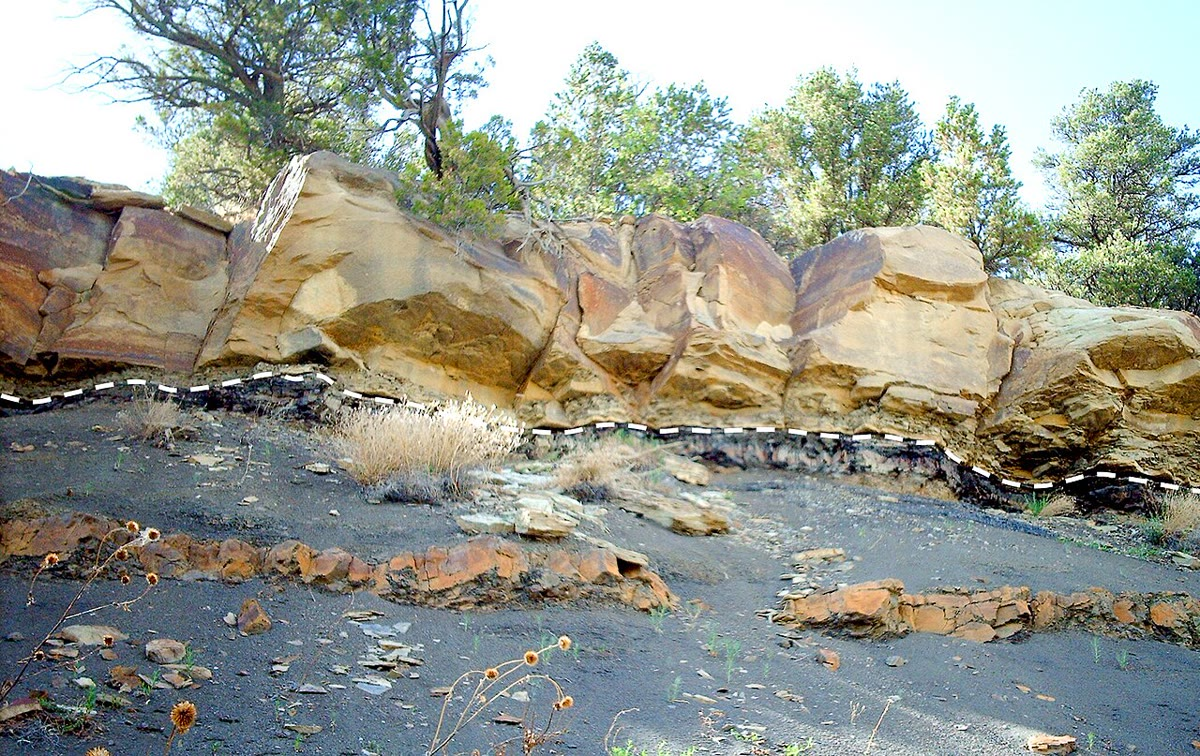
\includegraphics[width=0.78\linewidth]{images/book3/b1-kpg-boundary-trinidad.jpg}

{\small الحدّ بين الطباشيري والباليوجين، مُعلَّمًا بالخط المتقطّع، في متنزه بحيرة ترينيداد الحكومي بكولورادو: حجر رملي فوقه، وطبقات داكنة تحته وعلى طول الحدّ. (Nationalparks, CC~BY-SA~2.5, عبر Wikimedia Commons؛ الخط المتقطّع موجود في الأصل.)}
\label{fig:b1:stratigraphic-scale:kpg}
\end{omfigure}
% ledger: commons:kt-tlsp

\subsection*{نهاية البرمي}

كان الانقراض عند نهاية البرمي أشدّ فقد للحياة البحرية والبرّية في آخر نصف مليار سنة. وفي مَيشان بالصين، القطاع الذي يحوي GSSP لقاعدة الترياسي، أُرِّخت خمس طبقات رماد بطريقة اليورانيوم–الرصاص على الزركون. وتضعه بين \qty[uncertainty-mode=separate]{251.941(37)}{\Ma} و\qty[uncertainty-mode=separate]{251.880(31)}{\Ma}: فترة قدرها \num[uncertainty-mode=separate]{60 \pm 48} ألف سنة. ويسبقه انحراف سالب حادّ قدره \qty{3}{\permil} في نظائر الكربون في الكربونات، وظلّت دورة الكربون غير مستقرّة نحو \num{500} ألف سنة.
% ledger: burgess:end-permian, gssp:induan

قاعدة الترياسي نفسها، \qty[uncertainty-mode=separate]{251.902(24)}{\Ma}، لا تقع عند الانقراض، بل عند الظهور الأول للكونودونت \emph{Hindeodus parvus}، وهو مستوى يقع داخل فترة الانقراض المؤرّخة في مَيشان. فالانقراض مجموعة من الظهورات الأخيرة، يطمسها الحفظ؛ أما ظهور أول واحد لنوع معروف فيصنع خطًّا أكثر حدّة. وأسباب الانقراضين، أي الصدمة وأقاليم البازلت الكبرى، هي موضوع المجلد الثاني.
% ledger: gssp:induan, isg:biostratigraphy, burgess:end-permian

\section{المخطّط الدولي}\label{sec:b1:stratigraphic-scale:chart}

يجمع المخطط الكرونوستراتغرافي الدولي كل الوحدات، من الإيونوثيمات إلى الطوابق، في جدول واحد: أسماؤها، وأساس كل منها بالملايين من السنين مع عدم يقينه، وعلامة لكل أساس محدَّد ب GSSP مصادَق عليه، ولون معياري لكل وحدة، هو لون لجنة الخريطة الجيولوجية للعالم. ويُرسم جزء الفانيروزويك، مختزلًا إلى أحقابه وأدواره، أدناه من قيم المخطط نفسه.
% ledger: ics:base.Paleozoic, ics:colour.Paleozoic, gssp:count

\begin{omfigure}
\begin{tikzpicture}[font=\footnotesize]
\begin{axis}[y dir=reverse, ymin=0, ymax=538.8, xmin=0, xmax=6.2,
  width=6.6cm, height=11cm, scale only axis, clip=false,
  axis x line=none, axis y line*=left, ytick={0,100,...,500},
  ylabel={العمر (\unit{\Ma})}, tick label style={font=\scriptsize}]
  \pgfplotsinvokeforeach{Paleozoic,Mesozoic,Cenozoic,Cambrian,Ordovician,Silurian,Devonian,Carboniferous,Permian,Triassic,Jurassic,Cretaceous,Paleogene,Neogene,Quaternary}{
    \addplot[fill=ics#1, draw=black!70, line width=0.3pt] table[x=x, y=age] {figdata/out/bachelor-1-ics_chart-bar-#1.dat};}
  \addplot[draw=none, nodes near coords, point meta=explicit symbolic,
    every node near coord/.style={anchor=center, rotate=90, font=\scriptsize\bfseries}]
    coordinates {(0.5,395.351) [الباليوزويك] (0.5,158.951) [الميزوزويك] (0.5,33) [السينوزويك]};
  \addplot[draw=none, nodes near coords, point meta=explicit symbolic,
    every node near coord/.style={anchor=center, font=\scriptsize}]
    coordinates {(2,512.825) [الكمبري] (2,464.975) [الأوردوفيشي] (2,431.36) [السيلوري] (2,389.24) [الديفوني] (2,328.88) [الكربوني] (2,275.401) [البرمي] (2,226.651) [الترياسي] (2,172.25) [الجوراسي] (2,104.55) [الطباشيري] (2,44.52) [الباليوجين] (2,12.81) [النيوجين]};
  \addplot[mark=-, mark size=3pt, only marks, nodes near coords, point meta=explicit symbolic,
    every node near coord/.style={anchor=west, xshift=1pt, font=\scriptsize}]
    table[x=x, y=age, meta=lab] {figdata/out/bachelor-1-ics_chart-bases.dat};
  \addplot[only marks, mark=triangle*, mark size=3pt, mark options={rotate=90, fill=omThm, draw=omThm},
    nodes near coords, point meta=explicit symbolic,
    every node near coord/.style={anchor=west, xshift=3pt, font=\scriptsize, text=omThm}]
    coordinates {(4.75,251.902) [نهاية البرمي] (4.75,66) [نهاية الطباشيري]};
  \node[anchor=south, font=\scriptsize] at (axis cs:2,0) {الرباعي};
  \node[anchor=west, font=\scriptsize] at (axis cs:3.0,-14) {0};
  \node[anchor=south, font=\scriptsize\itshape] at (axis cs:0.5,-30) {حقب};
  \node[anchor=south, font=\scriptsize\itshape] at (axis cs:2,-30) {دور};
  \node[anchor=south, font=\scriptsize\itshape] at (axis cs:3.5,-30) {القاعدة (\unit{\Ma})};
\end{axis}
\end{tikzpicture}

{\small الفانيروزويك على المخطط الدولي: أحقابه الثلاثة واثنا عشر دورًا، بمقياس الرسم وبألوان المخطط، مع عمر قاعدة كل دور (عدم اليقين محذوف). وتميّز المثلثات القاعدتين اللتين تمثّلان أفقَي انقراض جماعي. والرباعي، طوله \qty{2.58}{\Ma}، هو الشريط الرفيع في الأعلى.}
\label{fig:b1:stratigraphic-scale:chart}
\end{omfigure}
% computed in figdata/bachelor-1/ics_chart.py; ledger: ics:base.Cambrian, ics:colour.Cambrian (every ics base and colour row of the eras and periods), burgess:end-permian, alvarez:iridium

الفترات غير متساوية بشدّة. فالطباشيري استمرّ \qty{77.1}{\Myr}، والنيوجين \qty{20.46}{\Myr}، والرباعي \qty{2.58}{\Myr} فقط؛ ومتوسط الاثني عشر هو \qty{44.9}{\Myr}. وهذه اللامساواة موروثة: فقد سُمِّيت الأنظمة في التصنيفات الأولى، قبل أن يُؤرَّخ أيّ صخر بالسنين. فبعض الأسماء يعطي موضعًا (الباليوجين، النيوجين، الرباعي)، وبعضها صخرًا (الكربوني، الطباشيري)، وبعضها شعبًا أو مكانًا (الأوردوفيشي، السيلوري، الديفوني، البرمي)، ويحتفظ المخطط بالأسماء بينما يعرّف قواعدها ب GSSP. أما الأعمار بالسنين فتأتي من التأريخ النظائري للصخور البركانية قرب الحدود، مثل طبقات الرماد في مَيشان (\cref{ch:b1:radiometric-methods})، المستكملة كما في \cref{prop:b1:stratigraphic-scale:interpolation}؛ وقد تُزيح نسخة جديدة من المخطط عمرًا بينما تبقى GSSP في مكانها.
% ledger: ics:base.Cretaceous, ics:base.Neogene, ics:base.Quaternary, isg:chronostratigraphy, burgess:end-permian

\begin{dated}{2024}
% ledger: iugs:anthropocene
الأنثروبوسين، وهو اسم اقتُرح عام 2001 لفترة جديدة يطبعها النشاط البشري، درسته منذ 2009 مجموعة عمل تابعة للّجنة الفرعية للطبقات الرباعية. وفي أواخر 2023 اقترحت \omterm{def:b1:stratigraphic-scale:lithostratigraphy}{المجموعة} سلسلة تبدأ نحو عام 1950، و GSSP لها في رسوب بحيرة كروفورد بأونتاريو. وصوّتت اللجنة الفرعية، وأُغلق التصويت في 4 مارس 2024، فرفضته: 4 أصوات مع، و\num{12} ضدّ، و\num{3} امتناعات، و\num{3} أعضاء لم يُصوّتوا. واعترف الأعضاء المصوّتون في اللجنة الدولية لعلم الطبقات بالتصويت. والأنثروبوسين ليس وحدة من المخطط؛ وهو يبقى مصطلحًا غير رسمي، شائع الاستعمال.
\end{dated}

\section{التمارين}

\begin{exercise}[$\star$]\label{exo:b1:stratigraphic-scale:1}
حدّد أيّ اسم هو لوحدة صخرية أو بيوستراتغرافية أو كرونوستراتغرافية أو جيوكرونولوجية، وأعطِ رتبتها حيث تكون لها رتبة: (أ)~نظام الجوراسي؛ (ب)~تكوين مردون الصخري؛ (ج)~الكرتاسي المبكّر؛ (د)~حيّز \emph{Hindeodus parvus}؛ (ه)~طابق الدانيان؛ (و)~حقبة الباليوسين؛ (ز)~عضو حجر رملي من مردون الصخري.
% ledger: isg:lithostratigraphy, isg:biostratigraphy, isg:chronostratigraphy
\end{exercise}

\begin{exercise}[$\star$]\label{exo:b1:stratigraphic-scale:2}
بأسس الحقب في شكل المخطط (أي الكمبري والترياسي والباليوجين)، احسب مدّة الباليوزويك والميزوزويك والسينوزويك، وحصّة كل منها من الفانيروزويك. وأيّ حصّة من الزمن منذ أساس الهاديان، \qty{4567}{\Ma}، يمثّل الفانيروزويك كلّه؟
% ledger: ics:base.Paleozoic, ics:base.Mesozoic, ics:base.Cenozoic, ics:base.Hadean
\end{exercise}

\begin{exercise}[$\star$]\label{exo:b1:stratigraphic-scale:3}
يُظهر جرف من الأسفل: الطبقات A وB وC وD، مائلة بزاوية \ang{40}؛ وجدارًا E يقطع A إلى D؛ وسطح تآكل يقطع قمّة D والجدار؛ وطبقات أفقية F وG فوقه؛ وصدعًا يزيح A إلى F دون G. رتّب الأحداث، وسمِّ المبدأ الذي يبرّر كل خطوة.
\end{exercise}

\begin{exercise}[$\star$]\label{exo:b1:stratigraphic-scale:4}
طبقتا رماد تبعدان \qty{30}{m} في صفيحة طينية أُرِّختا ب\qty{85.40}{\Ma} (الأسفل) و\qty{84.60}{\Ma} (الأعلى). والظهور الأول لحفرية دليلية يقع \qty{12}{m} فوق الرماد الأسفل. احسب معدّل التراكم وعمر الظهور الأول، بافتراض أن المعدّل ثابت.
\end{exercise}

\begin{exercise}[$\star\star$]\label{exo:b1:stratigraphic-scale:5}
في قطاع، لأربعة تصنيفات المدى التالي (بالأمتار): A من 0 إلى 34، وB من 12 إلى 50، وC من 26 إلى 62، وD من 41 إلى 70. (أ)~ارسم مخطط المدى. (ب)~أعطِ امتداد وسماكة \omterm{def:b1:stratigraphic-scale:biozone}{حيّز المدى} المتزامن لB وC، وسماكة \omterm{def:b1:stratigraphic-scale:biozone}{الحيّز الفاصل} بين الظهورين الأولين لB وD. (ج)~في قطاع ثانٍ يوجد B من 3 إلى \qty{15}{m}، وC من 9 إلى \qty{22}{m}، ولا شيء آخر معروف. أيّ حدود حيّزات (ب) يمكن التعرّف عليها هناك، وأيّها لا يمكن؟ وأيّ الآفاق يمكن ترابطها بين القطاعين بأكبر ثقة؟
\end{exercise}

\begin{exercise}[$\star\star$]\label{exo:b1:stratigraphic-scale:6}
خلال تجاوز بحري تحرّك الشاطئ نحو اليابسة بمعدّل \qty{20}{km} لكل مليون سنة. (أ)~بكم يختلف عمر قمّة الحجر الرملي الشاطئي بين بئرين تبعد كل منهما \qty{60}{km} عن الأخرى على امتداد اتّجاه التجاوز؟ (ب)~يسقط رماد بعد مليون سنة من مرور الشاطئ بالبئر الأبعد نحو البحر، حيث يتراكم طين البحر المفتوح بمعدّل \qty{30}{m} لكل مليون سنة. على أيّ ارتفاع فوق قمّة الحجر الرملي يُعثر على طبقة الرماد هناك؟ (ج)~أين كان الشاطئ حين سقط الرماد؟ وهل يوجد الرماد فوق الحجر الرملي أم تحته في البئر البرّي، ولماذا قد لا يُوجد فيه أصلًا؟ اشرح برسم تخطيطي.
\end{exercise}

\begin{exercise}[$\star\star$]\label{exo:b1:stratigraphic-scale:7}
(أ)~احسب عدم اليقين النسبي لعمري قاعدة اللوكوفيان (\qty[uncertainty-mode=separate]{419.62(136)}{\Ma}) والإنديان (\qty[uncertainty-mode=separate]{251.902(24)}{\Ma})، بالمئة. واقترح لماذا يختلفان كثيرًا. (ب)~من العمرين اللذين يحيطان بانقراض نهاية البرمي في مَيشان، \qty[uncertainty-mode=separate]{251.941(37)}{\Ma} و\qty[uncertainty-mode=separate]{251.880(31)}{\Ma}، أعِد حساب مدّة الانقراض وعدم يقينها، بافتراض أن الخطأين مستقلّان. قارن بالقيمة المنشورة \num[uncertainty-mode=separate]{60 \pm 48} ألف سنة.
% ledger: ics:base.Devonian, gssp:induan, burgess:end-permian
\end{exercise}

\begin{exercise}[$\star\star$]\label{exo:b1:stratigraphic-scale:8}
خذ \omterm{def:b1:comparative-planetology:small-bodies}{الكويكب} في عام 1980 كرةً عرضها \qty{10}{km}، كثافتها \qty{3000}{kg.m^{-3}} (قيمة مفترضة)، يقذف غبارًا كتلته 60 ضعف كتلته. (أ)~احسب كتلة \omterm{def:b1:comparative-planetology:small-bodies}{الكويكب} وكتلة الغبار. (ب)~وزّع الغبار بالتساوي على الأرض (القطر \qty{12756}{km}): أيّ كتلة تسقط على كل متر مربّع؟ (ج)~إن رُسِّب بكثافة \qty{2500}{kg.m^{-3}}، فكم سماكة الطبقة؟ (د)~كرّر (ج) لأقطار \qty{6}{km} و\qty{14}{km}، وهو مدى التقدير. قارن بسماكة طين الحدّ عند GSSP الدانيان.
% ledger: alvarez:iridium, planet:Earth.diameter, gssp:danian
\end{exercise}

\begin{exercise}[$\star\star$]\label{exo:b1:stratigraphic-scale:9}
(أ)~في قطاع مكثّف ترسّب فيه الرسوب بمعدّل \qty{2}{m} لكل مليون سنة، كم سماكة فترة \num{60} ألف سنة من انقراض نهاية البرمي؟ وكم تكون لأقصر مدّة وأطول مدّة يسمح بهما عدم يقينها؟ (ب)~في قطاع بحري عميق يتراكم بمعدّل \qty{10}{m} لكل مليون سنة، كم سماكة فترة \num{32000} سنة يتزامن ضمنها الاصطدام وحدّ K--Pg؟ (ج)~ماذا تقول هذه الأعداد عن أخذ عيّنات من قطاع لدراسة انقراض؟
% ledger: burgess:end-permian, renne:kpg
\end{exercise}

\begin{exercise}[$\star\star\star$]\label{exo:b1:stratigraphic-scale:10}
ينحدر سهل ساحلي بنسبة $1$ في $2000$، ويرتفع \omterm{def:b1:diagenesis-basins:eustasy}{مستوى البحر النسبي} بمقدار \qty{10}{m} لكل مليون سنة. (أ)~باستعمال \cref{prop:b1:stratigraphic-scale:transgression}، بأيّ سرعة يتحرّك الشاطئ نحو اليابسة، وبكم يختلف عمر قمّة حجر الشاطئ الرملي بين بئرين تبعد كل منهما \qty{30}{km} عن الأخرى؟ (ب)~يُوصَل الرسوب الآن إلى الشاطئ، فيبني السهل الساحلي نحو الأعلى بمقدار $a$ متر لكل مليون سنة عند الشاطئ. بيّن أن الشاطئ يتحرّك نحو اليابسة بمعدّل $(R - a)/s$ ما دام $a < R$. ماذا يحدث حين يكون $a > R$؟ (ج)~اشرح لماذا يمكن لقمّة حجر رملي يتغيّر عمرها بمليون سنة أن تبدو، في جرف واحد، تمامًا كسطح متساوي العمر.
\end{exercise}

\begin{exercise}[$\star\star\star$]\label{exo:b1:stratigraphic-scale:11}
طبقتا رماد تقعان على \qty{10}{m} و\qty{50}{m} في قطاع، وأُرِّختا ب\qty[uncertainty-mode=separate]{100.50(5)}{\Ma} و\qty[uncertainty-mode=separate]{99.70(3)}{\Ma}. (أ)~استكمل عمر مستوى على \qty{25}{m} وعدم يقينه ب\cref{prop:b1:stratigraphic-scale:interpolation}. (ب)~أين بين الرمادين يكون عدم اليقين أصغر ما يمكن؟ اعثر على قيمة $f$ التي تُصغّر $\sigma_t$، وعلى هذه القيمة الصغرى. (ج)~بيّن أن $\sigma_t$ لا يتجاوز أبدًا الأكبر من $\sigma_1$ و$\sigma_2$ بين الطبقتين.
\end{exercise}

\begin{exercise}[$\star\star\star$]\label{exo:b1:stratigraphic-scale:12}
تخترق بئر صفيحة طينية موحّدة. رماد أُرِّخ ب\qty{30.0}{\Ma} يقع على عمق \qty{1000}{m}، ورماد أُرِّخ ب\qty{29.0}{\Ma} على \qty{200}{m}؛ وحدّ طابق يقع على \qty{600}{m}. (أ)~استكمل عمره من الأعماق. (ب)~تراكمت الحبيبات، لا المسامات، بمعدّل ثابت. وباستعمال صخر الطين في \cref{tab:b1:diagenesis-basins:athy} و\cref{prop:b1:diagenesis-basins:solid}، احسب السماكة الصلبة بين كل رماد والحدّ، واستكمل العمر مرّة أخرى بنسبتها. (ج)~بكم ألف سنة يختلف التقديران، وأيّهما أفضل؟
% ledger: pybacktrack:compaction
\end{exercise}

\section{مسألة: ترابط ثلاثة قطاعات عبر حوض}

\begin{problem}[{مسألة نهاية الأسبوع --- كيف تجتمع الحفريات وطبقات الرماد والحجر الرملي متباين الزمن لتأريخ حدّ طابق}]
\label{pb:b1:stratigraphic-scale:1}
% values: calc/ch24.py; the basin, its sections, its taxa (Vardenoceras and Ostreola) and its ash ages are invented
تُسجَّل ثلاثة قطاعات على امتداد خطّ عبر حوض خيالي: A في الغرب، وB على بُعد \qty{25}{km} شرق A، وC على بُعد \qty{20}{km} شرق B. وفي كل منها يعلو حجرَ كِل الرملي تكوينُ مردون الصخري. والارتفاعات بالأمتار فوق قاعدة كل قطاع:
\begin{center}
\small
\begin{tabular}{lccc}
\hline
 & A & B & C \\
\hline
السماكة الكلية المسجّلة                       & 80.0 & 66.0 & 32.0 \\
قمّة حجر كِل الرملي                    & 45.0 & 20.0 & 6.0 \\
طبقة الرماد 1 (المؤرّخة ب \qty[uncertainty-mode=separate]{152.40(4)}{\Ma})       & 5.0  & 8.0  & 3.0 \\
طبقة الرماد 2 (المؤرّخة ب \qty[uncertainty-mode=separate]{151.20(4)}{\Ma})       & 71.0 & 56.0 & 27.0 \\
الظهور الأول ل \emph{Vardenoceras medium} & 36.6 & 31.2 & 14.8 \\
الظهور الأول ل \emph{Vardenoceras ultimum} & 65.8 & 52.0 & 24.8 \\
الظهور الأخير ل \emph{Vardenoceras primum}   & 49.0 & 40.0 & 19.0 \\
\hline
\end{tabular}
\end{center}
يُوجد \emph{V.~primum} من قاعدة كل قطاع. ويوجد الصدفي \emph{Ostreola} في حجر كِل الرملي وحده، في القطاعات الثلاثة كلها. وتُعرَّف ثلاثة حيّزات فاصلة: الحيّز~1 حتى الظهور الأول ل\emph{V.~medium}، والحيّز~2 حتى الظهور الأول ل\emph{V.~ultimum}، والحيّز~3 فوقه. ويُعرَّف حدّ \omterm{def:b1:stratigraphic-scale:chronostratigraphy}{الطابق}، بنموذجه الحدّي في موضع آخر، بالظهور الأول ل\emph{V.~medium}.

\medskip
\noindent\textbf{الجزء الأول --- الحيّزات الأحيائية.}
\begin{enumerate}
  \item ارسم القطاعات الثلاثة جنبًا إلى جنب بمقياس رأسي مشترك، مع حجر كِل الرملي وطبقات الرماد وحدود الحيّزات.
  \item أعطِ سماكة الحيّز~2 في كل قطاع، وسماكة الجزء من الحيّز~3 المسجَّل.
  \item لماذا لا يمكن وضع قاعدة الحيّز~1 في أيّ من القطاعات الثلاثة؟
  \item لماذا يكون \emph{Ostreola} حفرية دليلية ضعيفة، مهما كان شائعًا؟
  \item في أيّ حيّز يقع الظهور الأخير ل\emph{V.~primum} في كل قطاع؟ وهل يصلح حدًّا رابعًا للحيّزات؟
  \item رابِط القطاعات بالظهورين الأولين ل\emph{V.~medium} و\emph{V.~ultimum}. ماذا توحي نسبة سماكات الحيّز~2؟
\end{enumerate}

\noindent\textbf{الجزء الثاني --- حجر كِل الرملي.}
\begin{enumerate}[resume]
  \item في أيّ حيّز تقع قمّة حجر كِل الرملي في كل قطاع؟
  \item هل قمّة حجر كِل الرملي سطح متساوي العمر؟ في أيّ اتجاه تحرّك الشاطئ، وأيّ حدث هذا؟
  \item طبقة الرماد~1 تقع في حجر كِل الرملي في القطاعات الثلاثة كلها، وطبقة الرماد~2 في تكوين مردون الصخري. لماذا تكون طبقات الرماد خطوط زمن أفضل من حدّ \omterm{def:b1:stratigraphic-scale:lithostratigraphy}{التكوين}؟
  \item أيّ من مبادئ \cref{def:b1:stratigraphic-scale:principles} تبرّر تتبّع طبقة رماد واحدة من A إلى C؟
\end{enumerate}

\noindent\textbf{الجزء الثالث --- المعدّلات.}
\begin{enumerate}[resume]
  \item احسب معدّل التراكم بين طبقتي الرماد في كل قطاع، بالأمتار لكل مليون سنة.
  \item اقترح سبب هبوط المعدّل من A إلى C.
  \item كم سنة تمثّل عيّنة سماكتها \qty{10}{cm} في كل قطاع؟ وأيّ قطاع يعطي أدقّ دقّة زمنية؟
  \item بافتراض معدّلات ثابتة، احسب عمر قمّة حجر كِل الرملي في كل قطاع.
  \item احسب سرعة الشاطئ بين C وB، وبين B وA، بالكيلومترات لكل مليون سنة. هل أسرع التجاوز البحري أم أبطأ؟
  \item احسب عمر الظهور الأول ل\emph{V.~ultimum} في كل قطاع.
  \item هل تتفق الأعمار الثلاثة للسؤال~16 ضمن عدم يقين تأريخات الرماد؟ ماذا يقول هذا عن الظهور الأول؟
\end{enumerate}

\noindent\textbf{الجزء الرابع --- عمر الحدّ.}
\begin{enumerate}[resume]
  \item استكمل، في كل قطاع، عمر الظهور الأول ل\emph{V.~medium}.
  \item احسب عدم يقين كل عمر من عدم يقين تأريخات الرماد ب\cref{prop:b1:stratigraphic-scale:interpolation}.
  \item احسب متوسط الأعمار الثلاثة وانتشارها. هل الانتشار أكبر أم أصغر من عدم يقين السؤال~19؟
  \item في القطاع~A يقع الظهور الأول ل\emph{V.~medium} في حجر كِل الرملي، وفي B وC في تكوين مردون الصخري. كيف يمكن لتغيّر الصخرية بين طبقات الرماد أن ينحرف بالاستكمال في A؟
  \item أيّ القطاعات الثلاثة يصلح أفضل نموذجًا حدّيًّا، ولماذا؟ وأيّها أسوؤها؟
  \item كم دامت الحيّز~2؟
  \item ما عمر الحدّ المستكمل؟
\end{enumerate}
\end{problem}
